\documentclass{sigchi}

% Use this command to override the default ACM copyright statement (e.g. for preprints). 
% Consult the conference website for the camera-ready copyright statement.
\toappear{
	Submitted for review.
}

% Arabic page numbers for submission. 
% Remove this line to eliminate page numbers for the camera ready copy
\pagenumbering{arabic}


% Load basic packages
\usepackage{balance}  % to better equalize the last page
\usepackage{graphics} % for EPS, load graphicx instead
\usepackage{times}    % comment if you want LaTeX's default font
\usepackage{url}      % llt: nicely formatted URLs

% llt: Define a global style for URLs, rather that the default one
\makeatletter
\def\url@leostyle{%
  \@ifundefined{selectfont}{\def\UrlFont{\sf}}{\def\UrlFont{\small\bf\ttfamily}}}
\makeatother
\urlstyle{leo}


% To make various LaTeX processors do the right thing with page size.
\def\pprw{8.5in}
\def\pprh{11in}
\special{papersize=\pprw,\pprh}
\setlength{\paperwidth}{\pprw}
\setlength{\paperheight}{\pprh}
\setlength{\pdfpagewidth}{\pprw}
\setlength{\pdfpageheight}{\pprh}

% Make sure hyperref comes last of your loaded packages, 
% to give it a fighting chance of not being over-written, 
% since its job is to redefine many LaTeX commands.
\usepackage{hyperref}
\hypersetup{
pdftitle={Authorized Power Outlet},
pdfauthor={LaTeX},
pdfkeywords={SIGCHI, proceedings, archival format},
bookmarksnumbered,
pdfstartview={FitH},
colorlinks,
citecolor=black,
filecolor=black,
linkcolor=black,
urlcolor=black,
breaklinks=true,
}

% create a shortcut to typeset table headings
\newcommand\tabhead[1]{\small\textbf{#1}}


% End of preamble. Here it comes the document.
\begin{document}

\title{Authorized Power Outlet}

\numberofauthors{3}
\author{
  \alignauthor Ryan Fahsel\\
    \affaddr Georgia Institute of Technology\\
%    \affaddr{Address}\\
    \email ryan.fahsel@gatech.edu\\
%    \affaddr{Optional phone number}
  \alignauthor Colin Gray\\
    \affaddr Georgia Institute of Technology\\
%    \affaddr{Address}\\
    \email colin.gray@gatech.edu\\
%    \affaddr{Optional phone number}    
  \alignauthor Ramya Ramakrishnan\\
    \affaddr Georgia Institute of Technology\\
%    \affaddr{Address}\\
    \email rramakrishnan3@gatech.edu\\
%    \affaddr{Optional phone number}
}

\maketitle

\begin{abstract}

\end{abstract}

\keywords{
	NFC; RFID; Authorization.
%	\textcolor{red}{Mandatory section to be included in your final version.}
}

\category{K.6.5.}{}{}


\terms{
	Human Factors; Security. 
}

%See list of the limited ACM 16 terms in the
%instructions and additional information:
%\url{http://www.sheridanprinting.com/sigchi/generalterms.htm}.
%\textcolor{red}{Optional section to be included in your final version.}

\section{Introduction}

\subsection {Project Description}
The goal of this project is to expand on previous research in the area of NFC authorized power. The previous research done on NFC authorized power showed that using an NFC enabled device to control authorization to an outlet is possible; however, the prototype was very elementary (Fahsel 1). This project aims to make the device smaller, so that it is more reasonable to deploy in different settings. Also, the research will experiment with whether small wireless networks can be used to control networks of these NFC authorized outlets; this will be akin to how cordless phones in homes are all networked together through a base set. If this is realized, then microcontrollers might be able to be eliminated from the outlets, eliminating some of the space required by the outlet.  Additionally, NFC is not widely deployed yet, so the research aims to find a fallback way of generating authorization requests for smartphones that may not have NFC. Additionally, the prototype in the previous research did not have a way of detecting outlets that may have been left powered on, so the research will try to solve this problem. Lastly, the research will aim to find out whether it is possible to effectively track usage of equipment using these outlets. 

\subsection {Motivation}
The motivation for this project is to take a concept, authorized power, that has been proven and make it more practical.  This means making it smaller, so that it is easier to deploy. Also, authorized power means nothing if human error can leave the outlet on after the user has left. To increase the security of this concept, there needs to be a way to automatically turn the device off after the device has been inactive for a certain amount of time. Additionally, it seems that if people are going through the process of authenticating to a power outlet, it seems that the usage data should be logged because this gives the system timecard capabilities too without any extra hassle. Lastly, if this technology is to catch on, it needs to be usable by more than just NFC users because the set of people that use outlets is very widespread and diverse.

\section{Previous/Related Work}
We conducted previous work in this area to determine the effectiveness of using NFC for authorization. The results of this research were that the the NFC technology embedded in phones was an effective way to transmit the credentials of users. Each tool in the system was associated with an NFC sticker that was simple to use and worked well with the NFC embedded in the mobile device. The system could be easily implemented in a larger scale because phones with embedded NFC have become much more common and NFC stickers can be easily incorporated (Fahsel et al. 3).

Previous studies have also looked into using wireless networks to control some system. One study designed and implemented a wireless power outlet system in the home so that the outlets can be automatically controlled. It used a ZigBee radio as an actuator node for remote control. The results of the research were that this system was rather simple and flexible and was able to control many of the appliances in the house (Song et al. 1690). 

Another study analyzed how wireless devices can be used for controlling generic systems. In this work, input was received from a power source and multiple wireless devices in the system. A processor received many of these signals from the network and transmitted them to the output controller. This controller then used these signals to decide whether or not to provide power to some set of equipment (Myers and Higgins 1).

In another research work, Singhee designed a system that could intelligently exchange information between a system and its environment. He used the Nintendo Wii Remote as a way to transmit LED information. The results of the research was that a complex system was created with effective information flow. Although for the purposes of our work proposed here, we plan to have a simpler system (Singhee 199).

Several studies have also tracked usage of equipment, as we plan to do in this project. In one study, equipment usage was tracked in the hospital where RFID technology was being used to keep track of patients. The tracking was effective in preventing theft in the hospital (Wicks et al. 7). Similarly, in this project, we hope to track equipment usage, as that will provide more information about our system and its users.

As a whole, the previous work in this field has looked into using wireless networks for various applications, such as controlling home appliances and transmitting LED information. We hope to use similar wireless systems to control the network of outlets that we plan to use for authorization. Studies have also analyzed equipment usage, and we hope to implement a similar system to track usage of authorized tools.

\section{Our Work}

\subsection {Resources}
There are three main components to this project: an Android device, a webserver, and an Arduino controlled circuit. Additionally, we need an aesthetically pleasing and easy to use housing for the circuit.
\begin{itemize}
\item Android device: We own a Nexus 7 which is NFC enabled and a non-NFC enabled android phone.
\item Webserver: Georgia Tech offers free hosting to all students. We plan on using this to run a Fedora powered webserver with PHP, Python, and MySQL access.
\item RaspberryPi: We own a RaspberryPi that will be used as the base station to communicate with the nodes connected to the outlets.
\item Zigbee: We will need to order two Zigbees (\$25), which will be used for the communication between the nodes and the base stations.
\item Circuit Board: We plan to print a circuit board on the circuit board mill in the prototyping lab. We will need to order a few other components.
\item Housing: We will use the tools in the prototyping lab to create the case (possibly the 3d printer).
\end{itemize}

\subsection{Implementation}


%\begin{figure}[!h]
%\centering
%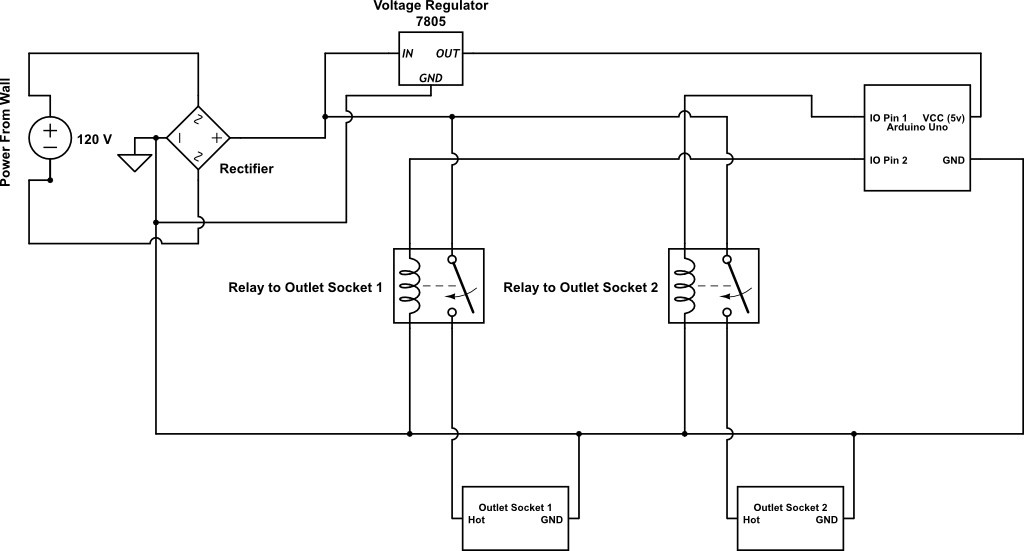
\includegraphics[width=0.9\columnwidth]{circuit}
%\caption{Circuit design.}
%\label{fig:circuit}
%\end{figure}

\subsection {Functionality}
The deliverable is a system that authorizes an outlet. It will try to implement all the optimizations described in the project description:
\begin{itemize}
\item Smaller form factor 
\item Personal area network to control network of outlets
\item Automatically turn off the outlet after period of inactivity
\item Usage tracking
\item Alternative way (non-NFC) to generate authorization requests
\end{itemize}

\section{Discussion}


\section{Future Work}


\section{Conclusion}


\section{References}
\begin{enumerate}
\item Fahsel, Ryan, Gray, Colin, and Ramakrishnan, Ramya. “NFC Authorized Outlet.” 2013.

\item Myers, Jenny, and Jim Higgins. "Method and system for using wireless devices to control one or more generic systems." U.S. Patent Application 09/854,870.

\item Singhee, Mukul. "A framework for the design of systems with intelligent and interactive information flow." (2010).

\item Song, Guangming, et al. "A wireless power outlet system for smart homes."Consumer Electronics, IEEE Transactions on 54.4 (2008): 1688-1691.

\item Wicks, Angela M., John K. Visich, and Suhong Li. "Radio frequency identification applications in hospital environments." Hospital topics 84.3 (2006): 3-9.
\end{enumerate}

\section{Acknowledgments}

We thank Dr. Gregory D. Abowd, Dr. Thad Starner, Clint Zeagler, and Caleb Southern for leading the class Mobile and Ubiquitous Computing, which was the inspiration for this project.

% Balancing columns in a ref list is a bit of a pain because you
% either use a hack like flushend or balance, or manually insert
% a column break.  http://www.tex.ac.uk/cgi-bin/texfaq2html?label=balance
% multicols doesn't work because we're already in two-column mode,
% and flushend isn't awesome, so I choose balance.  See this
% for more info: http://cs.brown.edu/system/software/latex/doc/balance.pdf
%
% Note that in a perfect world balance wants to be in the first
% column of the last page.
%
% If balance doesn't work for you, you can remove that and
% hard-code a column break into the bbl file right before you
% submit:
%
% http://stackoverflow.com/questions/2149854/how-to-manually-equalize-columns-
% in-an-ieee-paper-if-using-bibtex
%
% Or, just remove \balance and give up on balancing the last page.
%
\balance

% If you want to use smaller typesetting for the reference list,
% uncomment the following line:
% \small
%\bibliographystyle{acm-sigchi}
%\bibliography{sample}
\end{document}
